\documentclass[11pt,a4paper,fontset=windows]{ctexart}
% ===== 公共导言区：高等代数（一）期中模拟卷 =====
\usepackage{amsmath,amssymb}
\usepackage{unicode-math}
\setmathfont{TeX Gyre Termes Math}
\usepackage[margin=2.05cm,top=2.35cm,bottom=2.0cm,headsep=11pt,includefoot]{geometry}
\usepackage{fancyhdr}
\usepackage{lastpage}
\usepackage{enumitem}
\usepackage{array}
\usepackage{bm}
\usepackage{xcolor}
\usepackage{zhnumber}
\usepackage{needspace}

\definecolor{hdgray}{gray}{0.32}
\definecolor{lngray}{gray}{0.5}
\definecolor{notebg}{gray}{0.955}

\pagestyle{fancy}
\fancyhf{}
\renewcommand{\headrulewidth}{0.4pt}
\renewcommand{\footrulewidth}{0pt}
\fancyhead[L]{\small\color{hdgray}\songti 高等代数（一）\ 期中模拟试卷（\thepp）}
\fancyhead[R]{\small\color{hdgray}\songti 考试时间：120 分钟\quad 满分：100 分}
\fancyfoot[C]{\small\color{lngray}\songti 第 \thepage\ 页\quad 共 \pageref{LastPage}\ 页}

\setlength{\parindent}{0pt}
\setlength{\parskip}{2pt}
\linespread{1.16}

% 题目列表 1—8 连续编号
\newlist{qs}{enumerate}{1}
\setlist[qs]{label=\textbf{\arabic*.},ref=\arabic*,leftmargin=2.55em,
  labelsep=0.55em,itemsep=23pt,topsep=6pt,parsep=0pt}
\newlist{note}{enumerate}{1}
\setlist[note]{label=(\arabic*),leftmargin=1.75em,itemsep=1.5pt,topsep=2.5pt,parsep=0pt}
\newlist{sub}{enumerate}{1}
\setlist[sub]{label=(\arabic*),leftmargin=1.9em,itemsep=3pt,topsep=3pt,parsep=0pt}

\newcommand{\secA}[1]{\Needspace{9\baselineskip}\par\vspace{10pt}{\large\bfseries\songti #1}\par\vspace{3pt}\nopagebreak}
\newcommand{\blank}[1][2.6cm]{\underline{\hspace{#1}}}
\newcounter{pp}
\renewcommand{\thepp}{\chinese{pp}}

\setcounter{pp}{1}
\fancyhead[L]{\small\color{hdgray}\songti 高等代数（一）\ 专题讲义：多项式整除与单位根}
\fancyhead[R]{\small\color{hdgray}\songti 配合模拟卷（一）第 6 题}
\usepackage{tikz}

\newcommand{\sect}[1]{\Needspace{12\baselineskip}\par\vspace{16pt}%
  {\large\bfseries\songti #1}\par\vspace{3pt}\hrule height 0.6pt\par\vspace{8pt}}
\newcommand{\usub}[1]{\Needspace{6\baselineskip}\par\vspace{10pt}%
  {\normalsize\bfseries\songti #1}\par\vspace{2pt}}
\newcommand{\uex}[2]{\Needspace{9\baselineskip}\par\vspace{14pt}\noindent
  {\large\bfseries\songti 例~#1}\hfill{\small\color{hdgray}\songti #2}\par\vspace{2pt}%
  \hrule height 0.3pt\par\vspace{6pt}}
\newcommand{\uidea}[1]{\par\noindent{\small\songti\textbf{思路}\ \ #1}\par\vspace{3pt}}
\newcommand{\uann}[1]{\par\vspace{3pt}\noindent
  {\small\color{hdgray}\songti\textbf{批注}\ \ #1}\par\vspace{1pt}}
\newcommand{\uzz}{\textbf{证明：}}
\newcommand{\ujj}{\textbf{解：}}

\begin{document}

\begin{center}
{\LARGE\bfseries\songti 高等代数（一）· 专题讲义}\\[6pt]
{\LARGE\bfseries\songti 多项式整除与单位根}\\[8pt]
{\normalsize\songti 判断 $x^{a}\pm1$ 之间的整除关系，以及它们的最大公因式是什么}\\[2pt]
{\small\color{hdgray}\songti 配套：期中模拟卷（一）第 6 题；外校真题精选——多项式部分}
\end{center}
\vspace{-2pt}
\hrule height 0.5pt
\vspace{6pt}

{\small\songti
\textbf{本专题要解决的一件事：}给定 $x^{m}\pm1$ 与 $x^{n}\pm1$，谁整除谁？最大公因式是什么？
下面给出\textbf{一条直观}（单位圆上的正多边形）、\textbf{两套方法}（代根法、代数法）、
\textbf{七道例题}和\textbf{一张结论表}。结论表在第四节，可以先背下来再用。
}

%==================== 1 ====================
\sect{1\quad 单位根和它的“阶”}

\usub{1.1\quad 什么是单位根}

满足 $\zeta^{k}=1$（$k$ 为正整数）的复数 $\zeta$ 称为\textbf{单位根}。全部 $n$ 次单位根是
\[
\zeta_{k}=\mathrm{e}^{\frac{2k\pi\mathrm{i}}{n}}=\cos\frac{2k\pi}{n}+\mathrm{i}\sin\frac{2k\pi}{n},
\qquad k=0,1,\dots,n-1,
\]
共 $n$ 个，它们恰好是 $x^{n}-1=0$ 的全部根。例如 $n=4$ 时四个根是 $1,\ \mathrm{i},\ -1,\ -\mathrm{i}$。

\usub{1.2\quad “阶”是什么（本节唯一要记的东西）}

\textbf{定义：}使 $\zeta^{m}=1$ 成立的最小正整数 $m$，称为 $\zeta$ 的\textbf{阶}，记作 $\operatorname{ord}(\zeta)$。

阶为 $d$ 的单位根称为 \textbf{$d$ 次本原单位根}。例如：$1$ 的阶是 $1$；$-1$ 的阶是 $2$；
$\mathrm{e}^{2\pi\mathrm{i}/3}$ 与 $\mathrm{e}^{4\pi\mathrm{i}/3}$ 的阶都是 $3$；$\mathrm{e}^{\mathrm{i}\pi/3}$ 的阶是 $6$。

\smallskip
\textbf{一条等价关系（本专题所有推理的来源）：}
\[
\boxed{\ \zeta^{m}=1\iff \operatorname{ord}(\zeta)\mid m\ }
\]
它把“$\zeta$ 是某个多项式的根”翻译成“某个整数整除另一个整数”，于是整个问题变成算术题。

\smallskip
\textbf{怎么算阶：}若 $\zeta=\mathrm{e}^{2\pi\mathrm{i}r/s}$ 且 $(r,s)=1$，则 $\operatorname{ord}(\zeta)=s$。
所以判断阶只需把辐角写成“$\dfrac{2\pi\times(\text{分子})}{(\text{分母})}$”，分母就是阶。

\usub{1.3\quad 一条直观：单位圆上的正多边形（比公式好记）}

把 $x^{n}-1$、$x^{n}+1$ 的根画在单位圆上：

\begin{center}
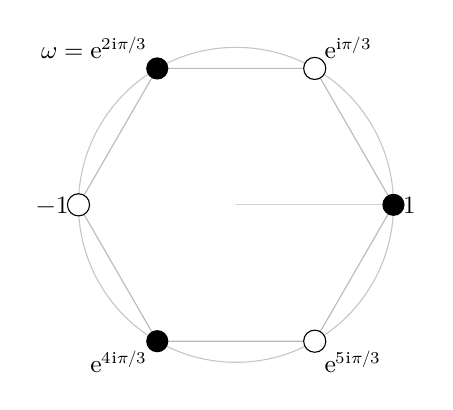
\begin{tikzpicture}[scale=2.0]
\draw[gray!45] (0,0) circle (1);
\draw[gray!35] (0,0) -- (1,0);
\foreach \k in {0,...,5}{\coordinate (P\k) at ({cos(60*\k)},{sin(60*\k)});}
\draw[gray!55] (P0)--(P1)--(P2)--(P3)--(P4)--(P5)--cycle;
\foreach \k in {0,2,4}{\fill (P\k) circle (2.0pt);}
\foreach \k in {1,3,5}{\draw[fill=white] (P\k) circle (2.0pt);}
\node[right] at (P0) {\small $1$};
\node[above right] at (P1) {\small $\mathrm{e}^{\mathrm{i}\pi/3}$};
\node[above left] at (P2) {\small $\omega=\mathrm{e}^{2\mathrm{i}\pi/3}$};
\node[left] at (P3) {\small $-1$};
\node[below left] at (P4) {\small $\mathrm{e}^{4\mathrm{i}\pi/3}$};
\node[below right] at (P5) {\small $\mathrm{e}^{5\mathrm{i}\pi/3}$};
\end{tikzpicture}
\end{center}

\centerline{\small\songti 图：正 $6$ 边形。\textbf{实心点}是 $x^{3}-1$ 的根，\textbf{空心点}是 $x^{3}+1$ 的根，两者交替分布。}

\smallskip
由此得到全专题最重要的一条几何直观：

\begin{center}
\renewcommand{\arraystretch}{1.45}
\begin{tabular}{@{}l l@{}}
$x^{n}-1=0$ 的根 & 正 $n$ 边形的\textbf{全部} $n$ 个顶点；\\[2pt]
$x^{n}+1=0$ 的根 & 正 $2n$ 边形顶点的\textbf{一半}——只取“隔一个算一个”的那些。\\[2pt]
\end{tabular}
\end{center}
理由：$x^{n}=-1\Rightarrow x^{2n}=1$，所以 $x^{n}+1$ 的根一定在正 $2n$ 边形上；而
$\bigl(\mathrm{e}^{k\pi\mathrm{i}/n}\bigr)^{n}=(-1)^{k}$，只有当 $k$ 是奇数时才等于 $-1$，
所以取的是\textbf{奇数位}顶点。

\uann{于是“两个多项式有没有公共根”就等于“两个正多边形有没有公共顶点”。第三节的例 3、例 4 全靠这条直观。}

%==================== 2 ====================
\sect{2\quad 两套方法、三件工具}

\usub{工具 1：换元 $t=x^{n}$}

若 $n\mid m$，令 $t=x^{n}$，则 $x^{m}-1=t^{\,m/n}-1$，可以直接用等比求和：
\[
t^{q}-1=(t-1)\bigl(t^{q-1}+t^{q-2}+\cdots+t+1\bigr).
\]
代回去就是本专题最常用的一个整除：
\[
\boxed{\ x^{n}-1\mid x^{qn}-1\ },\qquad\text{商为 }x^{n(q-1)}+x^{n(q-2)}+\cdots+x^{n}+1 .
\]
（例：$\dfrac{x^{3n}-1}{x^{n}-1}=x^{2n}+x^{n}+1$。）

\usub{工具 2：把“恰当的根”代进去（代根法）}

要证明 $f\mid g$，只要证明\textbf{$f$ 的每个根都被 $g$ 吃掉}；要证明 $f\nmid g$，
只要找到一个 $f$ 的根不被 $g$ 吃掉。这一出一进，是所有题目的核心。

\uann{关键是挑\textbf{阶最大}的那个根（本原根），阶越大，能推出整除条件越强。具体见例 1 的批注。}

\usub{工具 3：在指数上做辗转相除（代数法）}

把 $x^{n}-1\mid x^{qn}-1$ 用在带余除法 $m=qn+r$ 上：
\[
x^{m}-1=x^{r}\bigl(x^{qn}-1\bigr)+\bigl(x^{r}-1\bigr)
\ \Longrightarrow\
\bigl(x^{m}-1,\;x^{n}-1\bigr)=\bigl(x^{n}-1,\;x^{r}-1\bigr).
\]
指数对 $(m,n)\to(n,r)$，正是整数辗转相除的一步。

\usub{工具 4：先平方、再换元（处理“一减一加”）}

$D\mid x^{m}-1$ 且 $D\mid x^{n}+1$ 时，两边平方都变成“减号”：
\[
D\mid x^{2m}-1,\qquad D\mid x^{2n}-1 ,
\]
于是可以用现成的 $\bigl(x^{a}-1,x^{b}-1\bigr)=x^{(a,b)}-1$。这一招把“一减一加”化归成“两减”，见例 3 的方法二。

%==================== 3 例题 ====================
\sect{3\quad 例题}

%---- 例1
\uex{1}{整除判据\quad $x^{n}+1\mid x^{m}-1$ 什么时候成立}
设 $m,n$ 为正整数。证明：
\[
x^{n}+1\mid x^{m}-1\iff \frac{m}{n}\ \text{是正的偶数}.
\]

\uidea{整除 $\Rightarrow$ $x^{n}+1$ 的根都是 $x^{m}-1$ 的根。挑一个根代进去，让 $m,n$ 的关系露出来。}

\uzz
($\Leftarrow$) 设 $m=2kn$。令 $t=x^{n}$，则
\[
x^{m}-1=t^{2k}-1=(t^{2})^{k}-1 .
\]
被 $t^{2}-1=(t-1)(t+1)$ 整除，从而被 $t+1=x^{n}+1$ 整除。

\smallskip
($\Rightarrow$) 取 $\zeta=\mathrm{e}^{\mathrm{i}\pi/n}$。它满足
\[
\zeta^{n}=\mathrm{e}^{\mathrm{i}\pi}=-1,
\]
所以 $\zeta$ 是 $x^{n}+1$ 的根；由整除假设，$\zeta$ 也是 $x^{m}-1$ 的根，即 $\zeta^{m}=1$。而
\[
\zeta^{m}=\mathrm{e}^{\frac{\mathrm{i}\pi m}{n}} .
\]
这个数等于 $1$，当且仅当 $\dfrac{\pi m}{n}$ 是 $2\pi$ 的整数倍，即 $\dfrac{m}{n}$ 是偶数。
所以 $\dfrac{m}{n}=2k$，$m=2kn$。$\blacksquare$

\uann{为什么非取 $\zeta=\mathrm{e}^{\mathrm{i}\pi/n}$ 不可？它是 $x^{n}+1$ 里阶最大的根（阶为 $2n$）。
若随手取 $\zeta=-1$（阶为 $2$），只能得到“$2\mid m$”这种没用的弱条件。
用 $n=3,m=2$ 检验：$-1$ 是 $x^{3}+1$ 的根，且 $2\mid 2$ 成立，但 $x^{3}+1\nmid x^{2}-1$。可见取错根会得出错误结论。}

\smallskip
\textbf{另解（完全不用复数）}\quad 设 $m=qn+r$，$0\le r<n$。在 $x^{n}=-1$ 的意义下降次：
\[
x^{m}=x^{qn+r}=(x^{n})^{q}x^{r}\equiv(-1)^{q}x^{r}\pmod{x^{n}+1}.
\]
由 $x^{n}+1\mid x^{m}-1$ 得 $x^{m}\equiv1$，故 $x^{n}+1\mid(-1)^{q}x^{r}-1$。
但 $(-1)^{q}x^{r}-1$ 的次数是 $r<n$，比除式次数小，要能被整除只能恒等于零：
若 $q$ 为奇数它是 $-x^{r}-1\not\equiv0$；故 $q$ 为偶数，此时它为 $x^{r}-1$，恒为零要求 $r=0$。
于是 $m=qn$，$q=\dfrac{m}{n}$ 为偶数。$\blacksquare$

%---- 例2
\uex{2}{标准结论\quad $\bigl(x^{m}-1,\;x^{n}-1\bigr)=x^{d}-1$}
设 $m,n$ 为正整数，$d=(m,n)$。证明
\[
\bigl(x^{m}-1,\;x^{n}-1\bigr)=x^{d}-1 .
\]

\uidea{用工具 1 得到 $x^{n}-1\mid x^{qn}-1$，再用工具 3 在指数上做辗转相除。}

\uzz
\textbf{第一步（工具 1）。}对正整数 $q$，
\[
x^{qn}-1=(x^{n})^{q}-1=(x^{n}-1)\bigl(x^{n(q-1)}+x^{n(q-2)}+\cdots+x^{n}+1\bigr),
\]
故 $x^{n}-1\mid x^{qn}-1$。

\textbf{第二步（工具 3）。}设 $m=qn+r$，$0\le r<n$，则
\[
x^{m}-1=x^{r}\bigl(x^{qn}-1\bigr)+\bigl(x^{r}-1\bigr).
\]
求最大公因式时，“加上另一个多项式的倍数”不影响结果，而 $x^{r}(x^{qn}-1)$ 是 $x^{n}-1$ 的倍数，于是
\[
\bigl(x^{m}-1,\;x^{n}-1\bigr)=\bigl(x^{n}-1,\;x^{r}-1\bigr).
\]

\textbf{第三步（迭代）。}上式把指数对 $(m,n)$ 换成了 $(n,r)$，与整数辗转相除的一步完全相同。
反复进行，指数对最终变成 $(d,0)$，于是
\[
\bigl(x^{m}-1,\;x^{n}-1\bigr)=x^{d}-1 .\qquad\blacksquare
\]

\uann{两个“减号”的情形最简单：公因式永远存在，且只由 $d=(m,n)$ 决定。}

%---- 例3
\uex{3}{一减一加\quad $\bigl(x^{m}-1,\;x^{n}+1\bigr)$（本专题最难的一题）}
设 $m,n$ 为正整数，$e=(m,n)$。证明
\[
\bigl(x^{m}-1,\;x^{n}+1\bigr)=
\begin{cases}
x^{e}+1, & m\ \text{中 }2\ \text{的幂次比 }n\ \text{中多},\\[3pt]
1, & \text{否则}.
\end{cases}
\]
（记号：$v_{2}(k)$ 表示 $k$ 的质因数分解中 $2$ 的幂次，如 $v_{2}(12)=2$，“比 $n$ 多”即 $v_{2}(m)>v_{2}(n)$。）

\usub{方法一：看单位圆上两个正多边形的公共部分（最直观）}

\uidea{把 $x^{m}-1$ 的根看成正 $m$ 边形的顶点，$x^{n}+1$ 的根看成正 $2n$ 边形\textbf{奇数位}的顶点，
然后找两组顶点的公共部分。}

\ujj
\textbf{(1) 两个多边形共有的顶点。}正 $m$ 边形与正 $2n$ 边形的公共顶点，是正 $g=(m,\,2n)$ 边形的顶点，即 $\mathrm{e}^{2\pi\mathrm{i}l/g}$，$l=0,1,\dots,g-1$。
（理由：一个角要同时是 $\frac{2\pi}{m}$ 与 $\frac{2\pi}{2n}$ 的整数倍，那么它也一定是
$\frac{2\pi}{g}$ 的整数倍。）

\textbf{(2) 这些公共顶点在正 $2n$ 边形里排第几位？}由
\[
\mathrm{e}^{\frac{2\pi\mathrm{i}l}{g}}
=\mathrm{e}^{\frac{2\pi\mathrm{i}\,\cdot\,l(2n/g)}{2n}}
\]
可知它排在正 $2n$ 边形的第 $k=l\cdot\dfrac{2n}{g}$ 位。

\textbf{(3) 要求“奇数位”。}即要求 $k$ 为奇数：
\begin{itemize}[leftmargin=2em,itemsep=1pt,topsep=2pt]
\item 若 $\dfrac{2n}{g}$ 是\textbf{偶数}，则无论 $l$ 怎么取，$k$ 都是偶数，
      公共顶点全部落在正 $2n$ 边形的偶数位上，一个也取不到 $\Rightarrow$ \textbf{交集为空}；
\item 若 $\dfrac{2n}{g}$ 是\textbf{奇数}，取 $l$ 为奇数即可使 $k$ 为奇数 $\Rightarrow$ \textbf{有交集}，
      此时这样的 $l$ 正好有 $\dfrac{g}{2}$ 个，也就是 $x^{e}+1$ 的 $e=\dfrac{g}{2}$ 个根
      （因为 $v_{2}(m)>v_{2}(n)$ 时 $(m,2n)=2(m,n)$，即 $g=2e$）。
\end{itemize}

\textbf{(4) 把条件译成 $m,n$。}设 $m=2^{\alpha}m'$，$n=2^{\beta}n'$（$m',n'$ 为奇数），则
\[
\frac{2n}{g}=\frac{2^{\beta+1}n'}{2^{\min(\alpha,\beta+1)}\cdot(\text{奇数})}
\]
为奇数 $\iff \alpha\ge\beta+1\iff v_{2}(m)>v_{2}(n)$。

\textbf{(5) 收尾。}两个多项式都\textbf{无重根}（它们的导数与原式互素），所以“公共根集 $=x^{e}+1$ 的根集”
直接给出 $\bigl(x^{m}-1,x^{n}+1\bigr)=x^{e}+1$；交集为空时最大公因式为 $1$。$\blacksquare$

\usub{方法二：纯代数（不用复数，四步）}

记 $D=\bigl(x^{m}-1,\;x^{n}+1\bigr)$，$m=em_{1}$，$n=en_{1}$，其中 $e=(m,n)$，$(m_{1},n_{1})=1$。

\textbf{第 1 步（工具 4：平方对齐）。}$D\mid x^{m}-1\Rightarrow D\mid x^{2m}-1$；
$D\mid x^{n}+1\Rightarrow D\mid x^{2n}-1$。故
\[
D\mid\bigl(x^{2m}-1,\;x^{2n}-1\bigr)=x^{(2m,2n)}-1=x^{2e}-1=(x^{e}-1)(x^{e}+1).
\]

\textbf{第 2 步（排除 $x^{e}-1$ 那一半）。}断言 $\bigl(D,\;x^{e}-1\bigr)=1$：若不然，取公共根 $\zeta$，
则 $\zeta^{e}=1$；而 $x^{e}-1$ 是 $D$ 的因式、$D$ 又是 $x^{n}+1$ 的因式，故 $\zeta^{n}=-1$。但
\[
\zeta^{n}=(\zeta^{e})^{n_{1}}=1^{n_{1}}=1\neq-1,
\]
矛盾。于是由欧几里得引理（$(D,x^{e}-1)=1$ 且 $D\mid(x^{e}-1)(x^{e}+1)$）得
\[
D\mid x^{e}+1 .
\]

\textbf{第 3 步（换元 $y=x^{e}$）。}既然 $D\mid x^{e}+1$ 且 $D\mid x^{m}-1$，就有
\[
D\mid\bigl(x^{e}+1,\;x^{m}-1\bigr)=\bigl(y+1,\;y^{m_{1}}-1\bigr).
\]

\textbf{第 4 步（两句话算完）。}把 $y\equiv-1$ 代入即得带余除法
\[
y^{k}-1=(y+1)Q(y)+\bigl((-1)^{k}-1\bigr).
\]
\begin{itemize}[leftmargin=2em,itemsep=1pt,topsep=2pt]
\item $k$ 偶：余式为 $0$，故 $y+1\mid y^{k}-1$，$\bigl(y+1,y^{k}-1\bigr)=y+1$；
\item $k$ 奇：余式为 $-2$（非零常数），故互素，$\bigl(y+1,y^{k}-1\bigr)=1$。
\end{itemize}
取 $k=m_{1}$：若 $m_{1}$ 偶，则 $D=x^{e}+1$（此时 $n_{1}$ 必奇，$x^{e}+1\mid x^{n}+1$ 也成立）；
若 $m_{1}$ 奇，则 $D=1$。而 $m_{1}$ 偶 $\iff v_{2}(m)>v_{2}(n)$。$\blacksquare$

\uann{注意第 2 步的结论 $D\mid x^{e}+1$ 说明了这个最大公因式\textbf{只可能是 $x^{e}+1$ 或 $1$ 两种}，
不会出现“半个 $x^{e}+1$”这种复杂形状。}

%---- 例4
\uex{4}{两个加号\quad $\bigl(x^{m}+1,\;x^{n}+1\bigr)$}
设 $m,n$ 为正整数，$d=(m,n)$。证明
\[
\bigl(x^{m}+1,\;x^{n}+1\bigr)=
\begin{cases}
x^{d}+1, & v_{2}(m)=v_{2}(n),\\[3pt]
1, & v_{2}(m)\neq v_{2}(n).
\end{cases}
\]

\uidea{与例 3 同款，只是把“奇数位/偶数位”的条件换成“阶的 $2$ 的幂次”。}

\uzz
设 $\zeta$ 是公共根，$o=\operatorname{ord}(\zeta)$。由 $\zeta^{m}=-1$ 得
\[
o\mid 2m\quad\text{但}\quad o\nmid m ,
\]
这说明 $o$ 的 $2$ 的幂次恰好比 $m$ 的多一个：$v_{2}(o)=v_{2}(m)+1$。同理 $v_{2}(o)=v_{2}(n)+1$。
两式比较得必要条件
\[
v_{2}(m)=v_{2}(n).
\]
若这个条件成立，则 $d=(m,n)$ 与 $m,n$ 有相同的 $2$ 的幂次，于是
\[
\zeta^{m}=\zeta^{n}=-1\iff \zeta^{d}=-1 ,
\]
即公共根集恰为 $x^{d}+1$ 的根集；反之 $x^{d}+1$ 的每个根显然都是公共根。
故最大公因式为 $x^{d}+1$。条件不成立时不存在公共根，最大公因式为 $1$。$\blacksquare$

\uann{例：$\bigl(x^{3}+1,x^{9}+1\bigr)=x^{3}+1$（$d=3$，$v_{2}$ 都是 $0$）；
$\bigl(x^{4}+1,x^{6}+1\bigr)=1$（$v_{2}$ 分别为 $2,1$）。}

%---- 例5
\uex{5}{三个一次因式\quad $x^{2}+x+1\mid x^{2n}+x^{n}+1$}
设 $n$ 为正整数。证明：
\[
x^{2}+x+1\mid x^{2n}+x^{n}+1\iff 3\nmid n .
\]

\uidea{$x^{2}+x+1$ 的本原根是 $\omega=\mathrm{e}^{2\pi\mathrm{i}/3}$，阶为 $3$。按 $n\bmod 3$ 分成三类讨论。}

\uzz
设 $\omega=\mathrm{e}^{2\pi\mathrm{i}/3}$，则 $\omega^{3}=1$，$\omega\neq1$，且
\[
\omega^{2}+\omega+1=0 .
\]
记 $f(x)=x^{2n}+x^{n}+1$，则 $f(\omega)=\omega^{2n}+\omega^{n}+1$。

\textbf{若 $3\mid n$：}$\omega^{n}=1$，故 $f(\omega)=1+1+1=3\neq0$，$\omega$ 不是根，
故 $x^{2}+x+1\nmid f$。

\textbf{若 $3\nmid n$：}此时 $\omega^{n}$ 等于 $\omega$ 或 $\omega^{2}$（二者都是 $3$ 次本原单位根）。
而 $(\omega)^{2}=\omega^{2}$、$(\omega^{2})^{2}=\omega^{4}=\omega$，即“平方后变成另一个”，所以
$\omega^{2n}$ 与 $\omega^{n}$ 恰为 $\omega,\omega^{2}$ 各一个，于是
\[
f(\omega)=\omega^{2}+\omega+1=0 .
\]
又 $f(x)$ 是整系数多项式，其共轭 $\bar\omega=\omega^{2}$ 也是 $f$ 的根。
$x^{2}+x+1=(x-\omega)(x-\omega^{2})$ 无重根，故 $x^{2}+x+1\mid f$。$\blacksquare$

\uann{本质是“$\omega^{n}$ 只有三种可能（$1,\omega,\omega^{2}$），只有 $=1$ 那一种会失败”。
这个“按 $n$ 模 $3$ 分类”的框架，换成 $x^{2}-x+1$（根为 $6$ 次本原根）就是模 $6$ 分类。}

%---- 例6
\uex{6}{去掉公共部分后互素}
设 $m,n$ 为正整数，$d=(m,n)$。证明：
\[
\left(\frac{x^{m}-1}{x^{d}-1},\ \frac{x^{n}-1}{x^{d}-1}\right)=1 .
\]

\uidea{两个商都是“把公共的 $x^{d}-1$ 除掉”得到的，它们的根应该是各自剩下的那些。
只要证明两个根集不相交，再加上“无重根”即可。}

\uzz
记 $A=\dfrac{x^{m}-1}{x^{d}-1}$，$B=\dfrac{x^{n}-1}{x^{d}-1}$。两者都是 $x^{[m,n]}-1$ 的因式，
而后者无重根，所以 $A,B$ 都\textbf{无重根}。

设 $\zeta$ 是 $A,B$ 的公共根。由 $\zeta$ 是 $A$ 的根知 $\zeta^{m}=1$ 且
\[
\zeta^{d}\neq1
\]
（若 $\zeta^{d}=1$ 则 $\zeta$ 是 $x^{d}-1$ 的根，而 $A$ 与 $x^{d}-1$ 无公共根）。同理 $\zeta^{n}=1$。
于是
\[
\operatorname{ord}(\zeta)\mid (m,n)=d\ \Longrightarrow\ \zeta^{d}=1,
\]
与 $\zeta^{d}\neq1$ 矛盾。故 $A,B$ 没有公共根；又都无重根，所以 $(A,B)=1$。$\blacksquare$

\uann{这条结论很有用：它说明 $(x^{m}-1)(x^{n}-1)=(x^{d}-1)\bigl[x^{m}-1\ \text{与}\ x^{n}-1\ \text{的最小公倍式}\bigr]$，
且最小公倍式就是两个商之积。}

%---- 例7
\uex{7}{多个指数}
设 $n_{1},\dots,n_{s}$ 为正整数。证明
\[
\bigl(x^{n_{1}}-1,\ x^{n_{2}}-1,\ \dots,\ x^{n_{s}}-1\bigr)=x^{(n_{1},n_{2},\dots,n_{s})}-1 .
\]
并求 $\bigl(x^{12}-1,\ x^{18}-1,\ x^{30}-1\bigr)$。

\uidea{对 $s$ 归纳，每次用一次例 2。}

\uzz
$s=1$ 显然；$s=2$ 即例 2。设结论对 $s-1$ 成立，记 $d=(n_{1},\dots,n_{s-1})$，
$D=(d,n_{s})=(n_{1},\dots,n_{s})$。由例 2 及归纳假设，
\[
\bigl(x^{n_{1}}-1,\dots,x^{n_{s}}-1\bigr)=\bigl(x^{d}-1,\ x^{n_{s}}-1\bigr)=x^{(d,n_{s})}-1=x^{D}-1 .
\]
（求多个多项式的最大公因式可以先求前 $s-1$ 个，再与第 $s$ 个取，这是首一多项式下最大公因式的结合性。）

取 $n_{1}=12,\ n_{2}=18,\ n_{3}=30$：$(12,18)=6$，$(6,30)=6$，故所求为 $\;x^{6}-1$。$\blacksquare$

%==================== 4 结论表 ====================
\sect{4\quad 结论表（建议背下来）}

设 $d=(m,n)$，$v_{2}(k)$ 表示 $k$ 中质因数 $2$ 的幂次（$v_{2}(12)=2$，$v_{2}(9)=0$）。

\begin{center}
\renewcommand{\arraystretch}{1.9}
\begin{tabular}{@{}c|c|c@{}}
 & $x^{n}-1$ & $x^{n}+1$\\ \hline
$x^{m}-1$ & $x^{d}-1$\ \ （永远成立） & $x^{d}+1$\ \ 若 $v_{2}(m)>v_{2}(n)$，否则 $1$\\ \hline
$x^{m}+1$ & $x^{d}+1$\ \ 若 $v_{2}(n)>v_{2}(m)$，否则 $1$ & $x^{d}+1$\ \ 若 $v_{2}(m)=v_{2}(n)$，否则 $1$\\
\end{tabular}
\end{center}

\smallskip
\textbf{读表口诀：}
\begin{itemize}[leftmargin=2em,itemsep=2pt,topsep=2pt]
\item 两个都是“减号”：永远有公因式，就是 $x^{d}-1$，没有例外；
\item 一减一加：只有 $2$ 的幂次\textbf{更大}的那一边（“减号”所在那边）才拿得到 $x^{d}+1$；
\item 两个都是“加号”：必须两边的 $2$ 的幂次\textbf{相等}，才拿得到 $x^{d}+1$。
\end{itemize}

\smallskip
\textbf{用 $m=4,\ n=2$ 验一遍整张表}（$d=2$，$v_{2}(4)=2$，$v_{2}(2)=1$）：

\begin{center}
\renewcommand{\arraystretch}{1.6}
\begin{tabular}{@{}l l@{}}
$\bigl(x^{4}-1,\ x^{2}-1\bigr)=x^{2}-1$ & 第一行第一列，永远成立；\\[2pt]
$\bigl(x^{4}-1,\ x^{2}+1\bigr)=x^{2}+1$ & $2>1$ 成立；也可直接分解 $x^{4}-1=(x^{2}-1)(x^{2}+1)$；\\[2pt]
$\bigl(x^{4}+1,\ x^{2}-1\bigr)=1$ & $v_{2}(n)=1$ 不比 $v_{2}(m)=2$ 大，故为 $1$；\\[2pt]
$\bigl(x^{4}+1,\ x^{2}+1\bigr)=1$ & $2\neq1$，故为 $1$；注意 $x^{4}+1=(x^{2}+1)^{2}-2x^{2}$ 不可除。\\
\end{tabular}
\end{center}

\uann{四行都先用 SymPy 直接算过最大公因式，逐项一致。}

%==================== 5 易错点 ====================
\sect{5\quad 五个易错点}

\begin{enumerate}[leftmargin=2.2em,itemsep=7pt,topsep=3pt]
\item \textbf{“根集相同”推不出“整除”。}必须补一句“被除式无重根”。
例如 $x^{2}-1$ 与 $(x^{2}-1)^{2}$ 根集相同，但后者不整除前者。
本专题里的 $x^{n}\pm1$ 都无重根（其导数与原式互素），所以这条总是满足——但要写出来。

\item \textbf{求最大公因式时，不能只证明“有公共根”。}需要证明公共根集\textbf{正好}是某个多项式的根集
（例 3 的第 (3)(4) 步就是干这个）。只证“存在”只能回答“是否互素”。

\item \textbf{取根要取阶最大的（本原根）。}否则条件太弱。见例 1 的批注：取 $-1$ 只能得到 $2\mid m$。

\item \textbf{正 $2n$ 边形，不是正 $n$ 边形。}$x^{n}+1$ 的根在正 $2n$ 边形上，而且只占奇数位。
记成“正 $n$ 边形”会全错。

\item \textbf{$\dfrac{m}{n}$ 是整数，不等于 $\dfrac{m}{n}$ 是偶数。}例 1 的条件是后者。
例如 $m=3,n=1$：$m/n=3$ 是整数但是奇数，此时 $x+1\nmid x^{3}-1$。
\end{enumerate}

\vspace{12pt}
\hrule height 0.5pt
\vspace{4pt}
{\small\color{hdgray}\songti 小结：判断 $x^{a}\pm1$ 的整除关系，实质只有两步——
（1）把多项式放到单位圆上看正多边形；（2）比较两个多边形的公共顶点落在哪一半。
代数上对应的就是：把 $x^{a}\equiv\pm1$ 代进去降次，再比较次数或阶。}

\end{document}
